%%%%%%%%%%%%%%%%%%%%%%%%%%%%%%%%%%%%%%%%%
% CU Boulder Physics Lab Writeup One Column
% LaTeX Template
% Version 1.0 (2022-10-05)
%
% This template has been downloaded from:
% http://www.LaTeXTemplates.com
%
% Original author:
% Mathias Legrand (legrand.mathias@gmail.com) titled Stylish Article 
% With extensive modifications by:
% Vel (vel@latextemplates.com)
% Further modifications for CU Boulder Physics by:
% Kristopher Bunker (kristopher.bunker@colorado.edu)
%
% License:
% CC BY-NC-SA 3.0 (http://creativecommons.org/licenses/by-nc-sa/3.0/)
%
%%%%%%%%%%%%%%%%%%%%%%%%%%%%%%%%%%%%%%%%%

%----------------------------------------------------------------------------------------
%	PACKAGES AND OTHER DOCUMENT CONFIGURATIONS
%----------------------------------------------------------------------------------------

\documentclass[10pt]{PhysLab1C} % Document font size

\usepackage[english]{babel} % Specify a different language here - english by default

%----------------------------------------------------------------------------------------
%	COLUMNS
%----------------------------------------------------------------------------------------

\setlength{\columnsep}{0.55cm} % Distance between the two columns of text
\setlength{\fboxrule}{0.75pt} % Width of the border around the abstract

%----------------------------------------------------------------------------------------
%	COLORS
%----------------------------------------------------------------------------------------

\definecolor{color1}{RGB}{0,0,90} % Color of the article title and sections
\definecolor{color2}{RGB}{0,20,20} % Color of the boxes behind the abstract and headings

%----------------------------------------------------------------------------------------
%	HYPERLINKS
%----------------------------------------------------------------------------------------

\usepackage{hyperref} % Required for hyperlinks

\hypersetup{
	hidelinks,
	colorlinks,
	breaklinks=true,
	urlcolor=color2,
	citecolor=color1,
	linkcolor=color1,
	bookmarksopen=false,
	pdftitle={Title},
	pdfauthor={Author},
}

%----------------------------------------------------------------------------------------
%	LAB AND COURSE INFORMATION
%----------------------------------------------------------------------------------------

\CourseInfo{Electronics for the Physical Sciences \vert ~ \textbf{PHYS 3330}} %
\Department{\copyright \ Department of Physics \vert ~ \textbf{University of Colorado Boulder} \ \vert ~ \textbf{\today}} %
\Copyright{\today} %
\LabTitle{Filters} % Lab Title

%----------------------------------------------------------------------------------------
%	ABSTRACT
%----------------------------------------------------------------------------------------

\Abstract{\textbf{Lab 3:} Measuring the frequency dependence of low-pass, high-pass, and band-pass filters.}

%----------------------------------------------------------------------------------------

\begin{document}

\maketitle % Output the title and abstract box

%\tableofcontents % Output the contents section

\thispagestyle{firstpage} % Removes page numbering from the first page

%----------------------------------------------------------------------------------------
%	ARTICLE CONTENTS
%----------------------------------------------------------------------------------------

\section{Goals}

In this lab, you will characterize the frequency dependence of three passive filters. You will gain more experience modeling both the response of the filters and how your measurement tools affect your measurements.

Proficiency with new equipment:

\begin{itemize}
\item
  Oscilloscope probe
\item
  Capacitors and inductors

  \begin{itemize}
  \item
    Measure capacitance and inductance with an LCR meter
  \end{itemize}
\end{itemize}

Modeling the physical system:

\begin{itemize}
\item
  Develop mathematical models of frequency dependent voltage dividers
\end{itemize}

Modeling measurement systems:

\begin{itemize}
\item
  Refine the model of scope measurement tool to include capacitance of
  the coax cable
\item
  Refine the measurement system to reduce the effect of the capacitance
  of a coax cable
\end{itemize}

%------------------------------------------------

\section{Definitions}

\textbf{Scope probe} - a test probe used to increase the resistive
impedance and lower the capacitive impedance compared to a simple coax
cable probe.

\textbf{Transfer function} - the complex function \(V_{out}/V_{in}\).

\textbf{Gain} - the magnitude of the transfer function is the voltage
gain \(G=|T|=|V_{out}/V_{in}|\). The power gain is the square of this:
\(|V_{out}/V_{in}|^2\). If the gain is not specified, you can assume it
is the voltage (or amplitude) gain.

\textbf{Decibel (dB)} - a measure of the power transmitted by converting
the power gain (or voltage gain) to a logarithmic scale. The difference
in power between output and input in decibels (dB) is
\(10~log_{10}~|V_{out}/V_{in}|^2 =20~log_{10}~|V_{out}/V_{in}| \). One
common reference point is where the ratio of output to input power is
1/2, which is \(10~log_{10}(0.5) = -3~dB\). This corresponds to
\(|V_{out}/V_{in}| = 1/\sqrt 2 = 0.707 = 70.7\%\).

\textbf{Pass band} - the range of frequencies that can pass through a
filter without being attenuated.

\textbf{Attenuation band }- the range of frequencies where the filter
attenuates the signal.

\textbf{Cutoff frequency or corner frequency or 3 dB frequency, fc} -
frequency separating the pass and attenuation bands. It is the frequency
at the half-power (3 dB) point, where the \emph{power} transmitted is
half the maximum power transmitted. The output voltage \emph{amplitude}
at f = fc is $1/\sqrt{2} = 70.7\%$ of the maximum amplitude.

\textbf{Low-pass filter} - a filter that passes low frequency signals
and attenuates (reduces the amplitude of) signals with frequencies
higher than the cutoff frequency. Also known as an integrator.

\textbf{High-pass filter} - a filter that passes high frequency signals
and attenuates (reduces the amplitude of) signals with frequencies lower
than the cutoff frequency. Also known as a differentiator.

\textbf{Band-pass filter} - passes frequencies within a certain range
and attenuates frequencies outside that range.

\textbf{Band-pass filter bandwidth} - the range of frequencies between
the upper (\(f_+\)) and lower (\(f_-\)) half power (3dB) points:
\(\Delta f = f_+ - f_-\).

%------------------------------------------------

\section{Application of Filters}

A frequent problem in physical experiments is to detect an electronic
signal when it is hidden in a background of noise and unwanted signals.
The signal of interest may be at a particular frequency, as in an NMR
experiment, or it may be an electrical pulse, as from a nuclear particle
detector. The background generally contains thermal noise from the
transducer and amplifier, 60 Hz power pick up, transients from
machinery, radiation from radio and TV stations, cell phone radiation,
and so forth. The purpose of filtering is to enhance the signal of
interest by recognizing its characteristic time dependence and to reduce
the unwanted background to the lowest possible level. A radio does this
when you tune to a particular station, using a resonant circuit to
recognize the characteristic frequency. The signal you want may be less
than 10\textsuperscript{-6} of the total radiation power at your
antenna, yet you get a high-quality signal from the selected station.
Many experiments require specific filters designed so that the signal
from the phenomenon of interest lies in the pass-band of the filter,
while the attenuation bands are chosen to suppress the background and
noise.

This experiment introduces you to the filtering properties of some
widely used but simple circuits, employing only a resistor and capacitor
for high- and low-pass filters and an LCR (inductor, capacitor,
resistor) circuit for a band-pass filter.

%------------------------------------------------

\section{Filter Basics}

Whenever we discuss frequency in the lab, measured in Hz, we mean $f$,
and this is the most relevant. However, to avoid a bunch of factors of
$2\pi$, the angular frequency $\omega$ often appears in theoretical derivations.
Just remember that $\omega = 2\pi f$ so it is easy to convert. You should show
results versus $f$.

\subsection{RC low- and high-pass filters}

The response of RC low-pass and high-pass filters to sine waves is
discussed in Steck 2.3.5 \& 2.3.7, H\&H 1.18-\/-1.19, and Fischer-Cripps
3.9-\/-3.10. For these circuits, the magnitudes of the transfer
functions are:

\[\left| T(f) \right| = \frac{1}{\sqrt{1 + (2\pi fRC)^{2}}} 
~~~\mbox{(low-pass)}
\]

\[\left| T(f) \right| = \frac{2\pi fRC}{\sqrt{1 + (2\pi fRC)^{2}}}
~~~\mbox{(high-pass)}\]

For both filters: \(f_{C} = 1/{2\pi RC}\ \), where \(f_{C}\) is the
frequency at which the power drops by 3 dB (which means it is half of
the maximum). In this lab, we are finding how efficiently signals of
different frequencies are passed. This is called the frequency domain.
Later, we will look at the time domain, where we see how the output
changes as a function of time. In that context, low-pass and high-pass
filters are called integrators and differentiators.

\subsection{Parallel LRC band-pass filters}

The LCR circuit is described in Fischer-Cripps 3.12, H\&H 1.22, and
Steck 2.6 (note that the Steck example is for a \emph{serial} LCR
circuit so the concepts are the same but the details are different). As
this is another generalized voltage divider,

\[V_{out} = V_{in} = IZ_{2} = V_{in}\frac{Z_{2}}{Z_{1} + Z_{2}} \]
\[Z_{1} = R\]
\[Z_{2} = \frac{j\omega L}{1 - \omega^{2}LC}\]

The magnitude of the transfer function can then be calculated as:

\[\left| T(\omega) \right| = \sqrt{\frac{V_{out}V_{out}^{*}}{V_{in}V_{in}^{*}}}\]

where \(*\) indicates the complex conjugate. The algebra is left for you
as a prelab exercise.

The resonant frequency, $f_0$ and $Q$ factor (quality factor) are given by:

\[f_{0} = \frac{1}{2\pi\sqrt{LC}}\]
\[Q = \omega_{0}RC = \frac{R\sqrt{C}}{\sqrt{L}} = \frac{f_{0}}{\Delta f}\]

The resonant frequency, \(f_{0}\), is the center frequency of the pass
band, and \(Q\) is equal to the ratio of the center frequency to the
bandwidth \(\Delta f\). (These definitions are exactly true only for
\(Q\gg1\)).

For a resonant LCR circuit the characteristic impedance, \(Z_0\), is the
magnitude of the impedance of the inductor or the capacitor at the
resonant frequency:

\[Z_{0} = \omega_{0}L = \frac{1}{\omega_{0}C} = \frac{\sqrt{L}}{\sqrt{C}}\]

%------------------------------------------------

\section{Useful Readings}

\begin{enumerate}
\item
  \href{https://atomoptics-nas.uoregon.edu/~dsteck/teaching/electronics/electronics-notes.pdf}{Steck} Sections 2.1, 2.3, 2.4, 2.6
\item
  Fischer-Cripps 3.4-3.18
\item
  Horowitz \& Hill 2\textsuperscript{nd} Ed. 1.13-1.24 (and Appendix A
  on scope probes)
\end{enumerate}

%------------------------------------------------

\section{Prelab}

Answer the following questions using Mathematica. Save the complete
notebook as a pdf and turn it in to Canvas by midnight the day before
your lab section meets. \textbf{Bring an electronic copy of your
notebook to lab, preferably on your own laptop. You will use it to plot
your data during the lab session.}

% \begin{figure}[h]%
%     \centering
%     \subfloat[\centering Low-pass filter]{{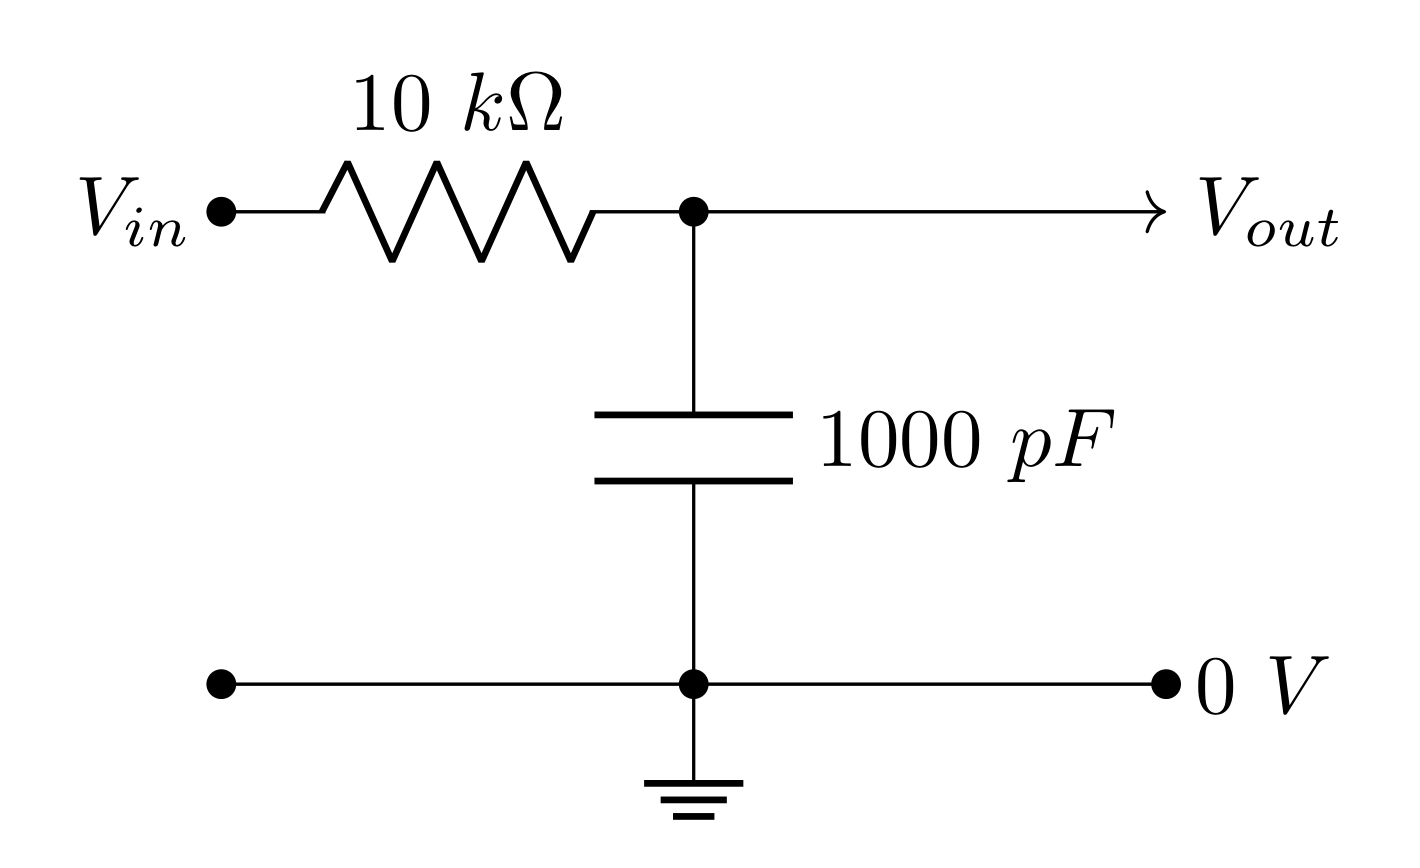
\includegraphics[width=5.5cm]{lab3fig/low-pass-1.png} } \label{low-pass-1}}%
%     %\qquad
%     \subfloat[\centering High-pass filter]{{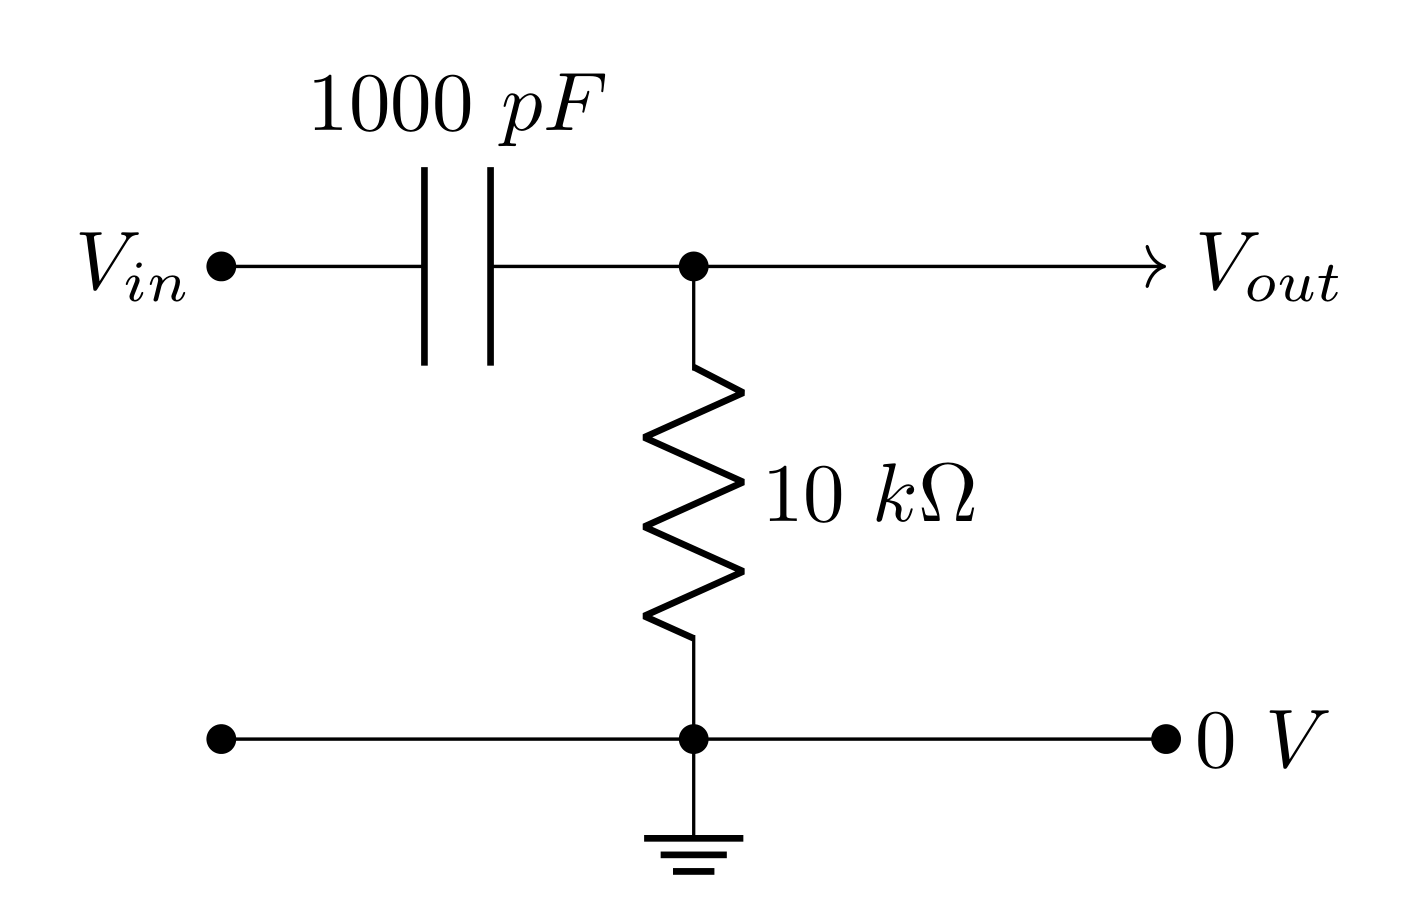
\includegraphics[width=5.5cm]{lab3fig/high-pass-1.png} }\label{high-pass-1}}%
%     %\qquad
%     \subfloat[\centering Band-pass filter]{{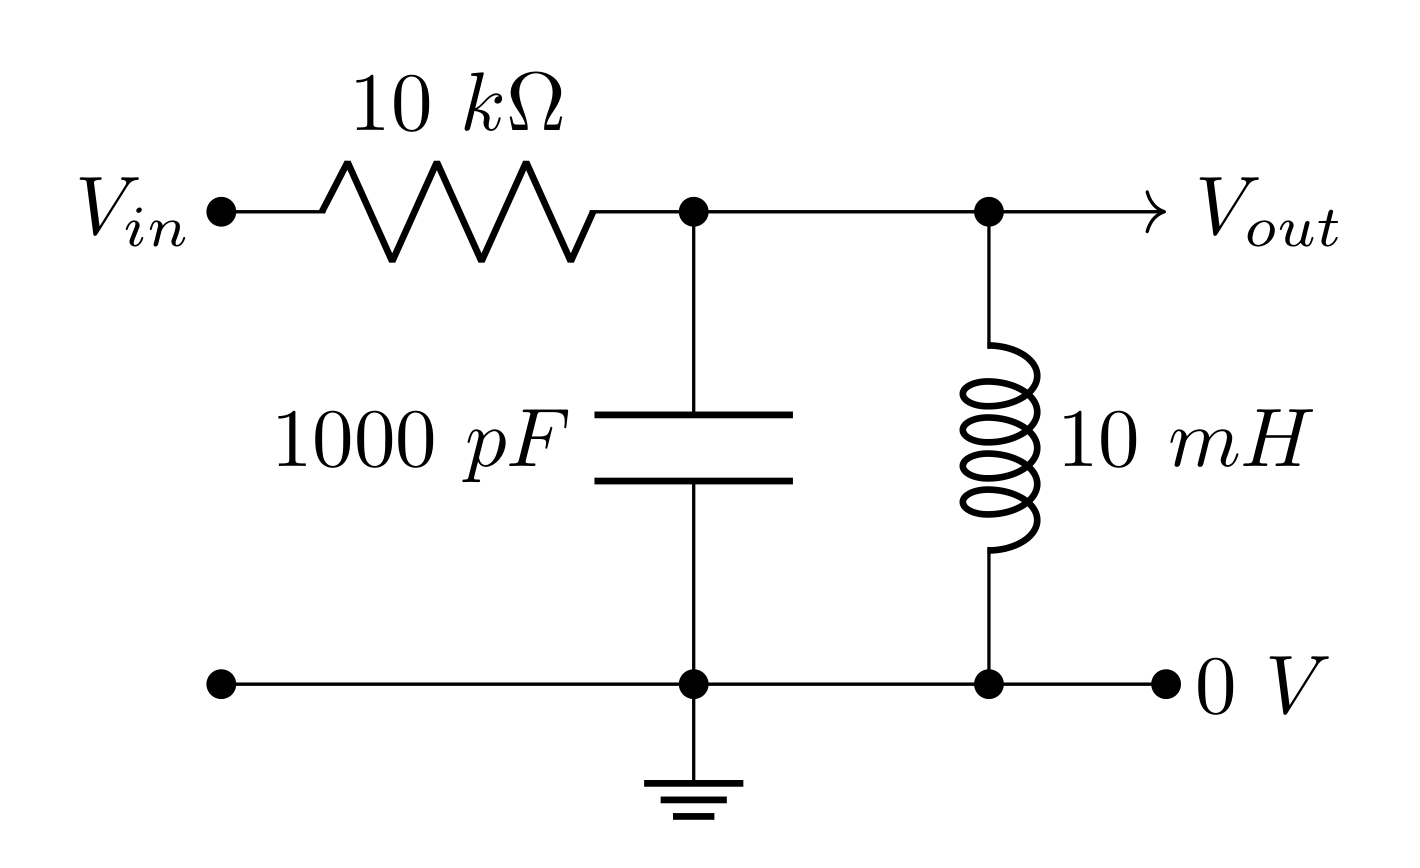
\includegraphics[width=5.5cm]{lab3fig/band-pass-1.png} }\label{band-pass-1}}%
%     \medskip
%     \caption{Filters}%
%     \label{filters}%
% \end{figure}

\begin{figure}[h]
     \centering
     \begin{subfigure}[b]{0.3\textwidth}
         \centering
         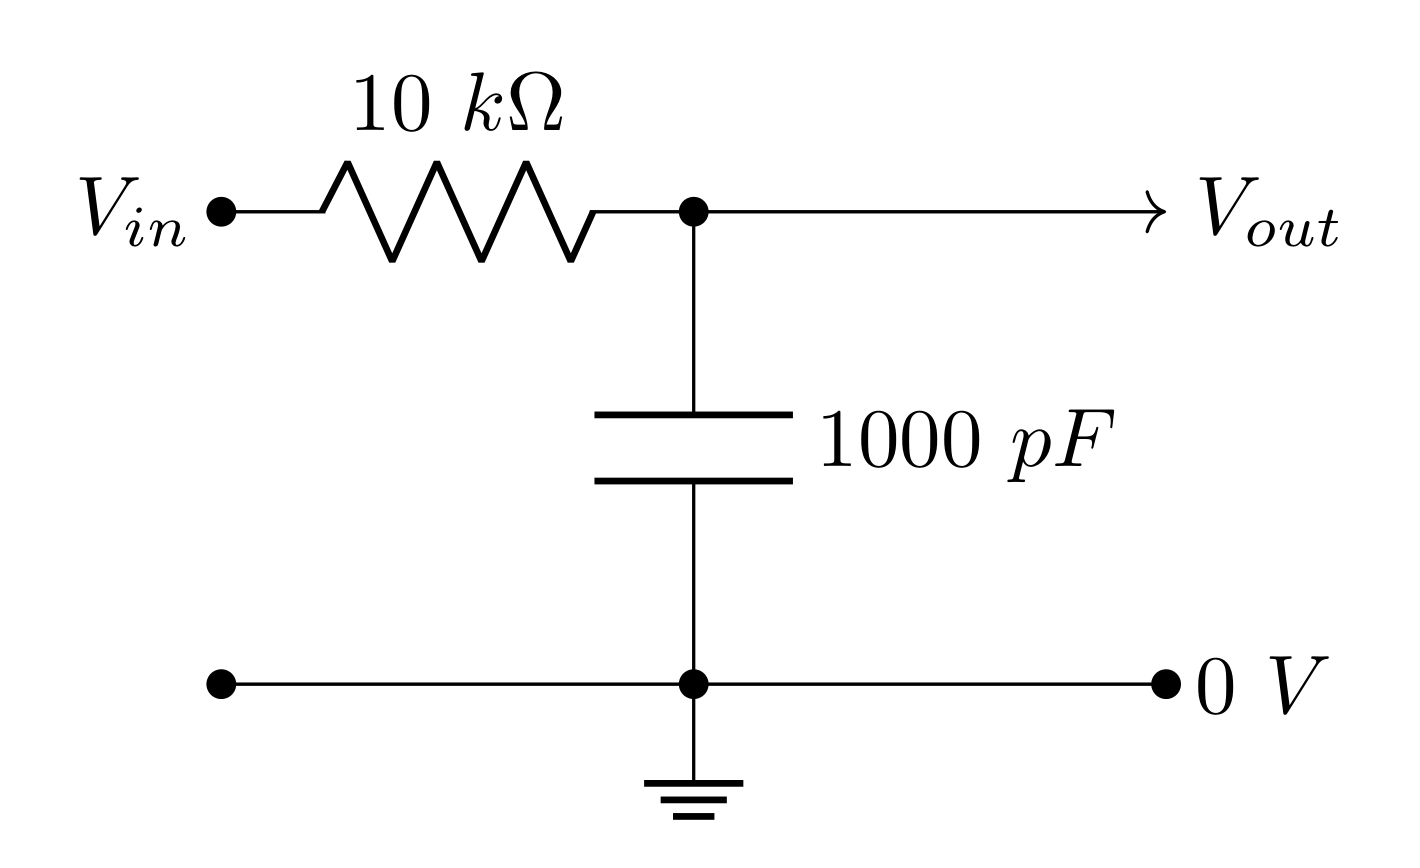
\includegraphics[width=\textwidth]{lab3fig/low-pass-1.png}
         \caption{Low-pass filter}
         \label{low-pass-1}
     \end{subfigure}
     \hfill
     \begin{subfigure}[b]{0.3\textwidth}
         \centering
         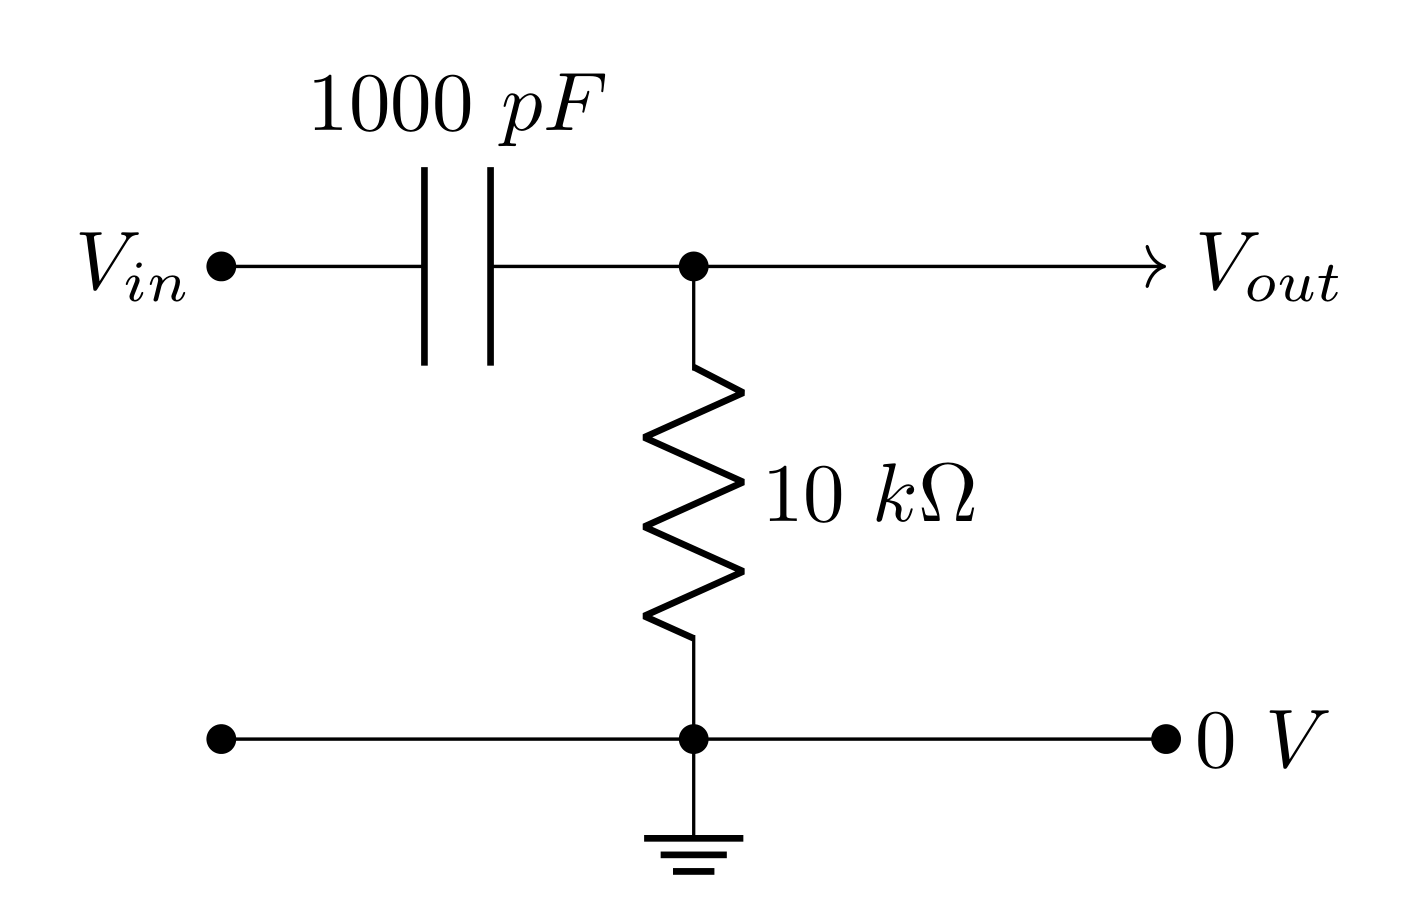
\includegraphics[width=\textwidth]{lab3fig/high-pass-1.png}
         \caption{High-pass filter}
         \label{high-pass-1}
     \end{subfigure}
     \hfill
     \begin{subfigure}[b]{0.3\textwidth}
         \centering
         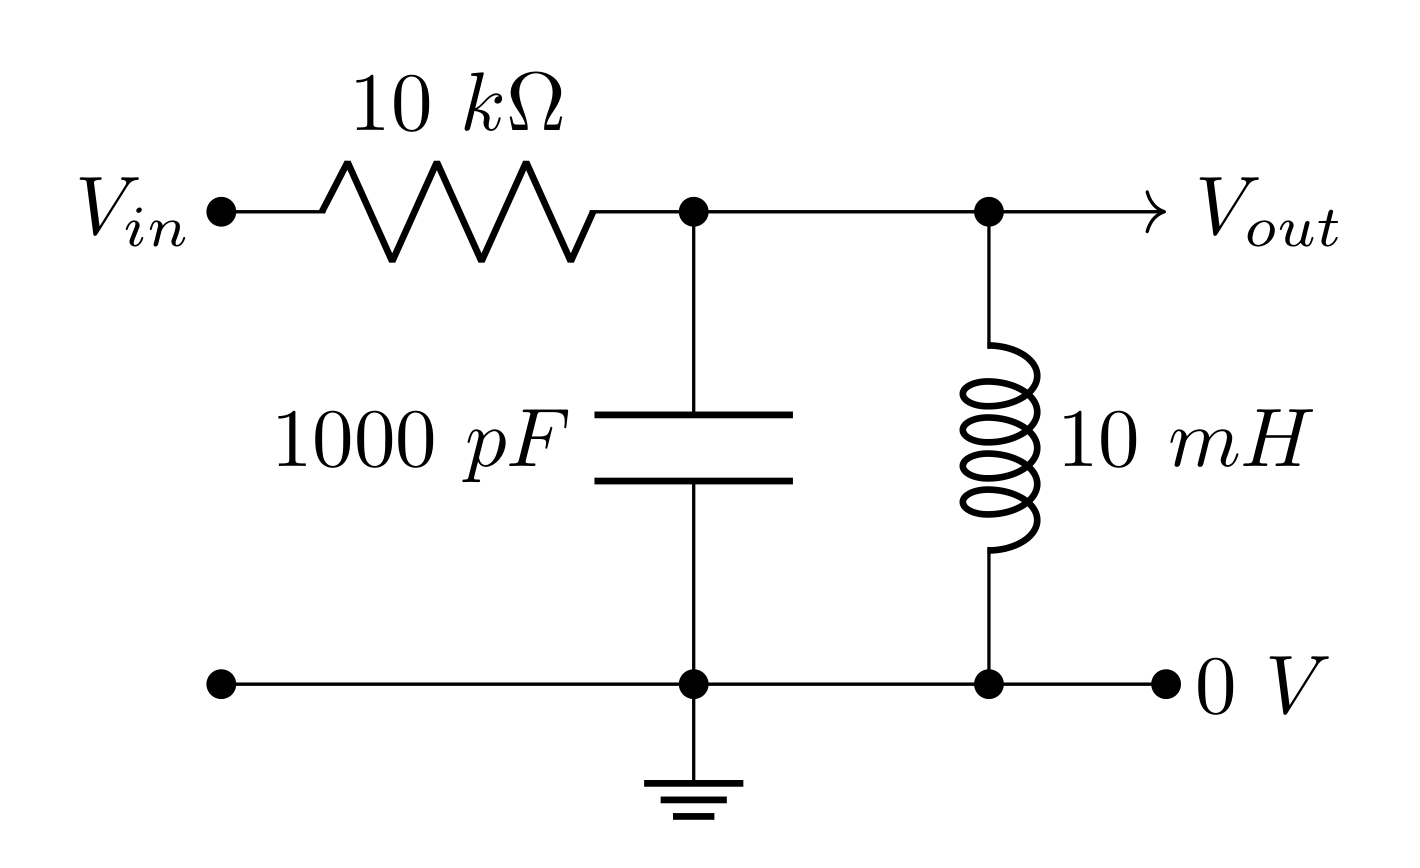
\includegraphics[width=\textwidth]{lab3fig/band-pass-1.png}
         \caption{Band-pass filter}
         \label{band-pass-1}
     \end{subfigure}
     \medskip
        \caption{Filters}
        \label{filters}
\end{figure}


% \begin{figure}[ht]
% \centering
% \begin{subfigure}[t]{0.3\textwidth}
% \centering
% \begin{circuitikz}[american voltages]
%     \draw (0,0) node[anchor = east]{$V_{in}$} to [R=$R$, l=$10~k\Omega$, *-*] ++(2,0) node{}
%         [->] (2,0) to ++(2,0) node[anchor = west]{$V_{out}$};
%     \draw (2,0) to [C=$C$, l=$1000~pF$, -*] (2,-2) node[ground]{};
%     \draw [short,*-] (0,-2) to (2,-2)
%         to [short,-*](4,-2) node[anchor = west]{$0~V$};
% \end{circuitikz}
%  \caption{low-pass}
%  \label{low-pass-1}
%  \end{subfigure}
%  \hspace{0.75cm}%
%  \begin{subfigure}[t]{0.3\textwidth}
% \centering
% \begin{circuitikz}[american voltages]
%     \draw (0,0) node[anchor = east]{$V_{in}$} to [C=$C$, l=$1000~pF$, *-*] ++(2,0)
%     [->] (2,0) to ++(2,0) node[anchor = west]{$V_{out}$};
%     \draw (2,0) to [R=$R$, l=$10~k\Omega$, -*] (2,-2) node[ground]{};
%     \draw [short,*-] (0,-2) to (2,-2)
%         to [short,-*](4,-2) node[anchor = west]{$0~V$};
% \end{circuitikz}
%  \caption{high-pass}
%  \label{high-pass-1}
%  \end{subfigure}
%  \hspace{0.75cm}%
%  \begin{subfigure}[t]{0.3\textwidth}
%  \centering
% \begin{circuitikz}[american voltages]
%     \draw (0,0) node[anchor = east]{$V_{in}$} to [R=$R$, l=$10~k\Omega$, *-*] ++(2,0) node{}
%         [->] (2,0) to ++(2,0) node[anchor = west]{$V_{out}$};
%     \draw (2,0) to [C=$C$, l_=$1000~pF$, -*] (2,-2) node[ground]{};
%     \draw [short,*-] (0,-2) to (2,-2)
%         to [short,-*](4,-2) node[anchor = west]{$0~V$};
%     \draw (3.25,0) to [L=$L$, l=$10~mH$, *-*] (3.25,-2);
% \end{circuitikz}
%  \caption{band-pass}
%  \label{band-pass-1}
%  \end{subfigure}
%   \medskip
%  \caption{Filters}
%  \label{filters}
%  \end{figure}


\subsection{Low- and high-pass filters}


\begin{enumerate}
\def\labelenumi{\arabic{enumi}.}
\item
  Define functions in Mathematica to calculate the cut-off or 3 dB
  frequency, \(f_c\), for the low- and high-pass filters in Figure \ref{low-pass-1} and \ref{high-pass-1}. The input parameters to this function should 
  be the resistance and capacitance of your circuit. Evaluate the
  functions using the nominal 
  values shown in the schematic. During the lab, you can input the exact
  values of your 
  components and thus quickly predict the 3 dB frequency you expect for
  your circuit.
\item
  Create two Bode plots (one for each filter) of the frequency response
  of the low-pass and
  high-pass filters in Figure \ref{filters}. A Bode plot is a log-log plot of the
  gain (\(V_{out}/V_{in}\)) versus
  frequency, similar to what is on pages 61 \& 62 of Steck (although the
  Steck plots have the
  x-axis in units of \(2\pi RC\) and you should use units of Hz). Make
  sure to include a large
  enough range in frequency to see both the pass and attenuation bands.
  Make sure to label
  your axes! Details about making plots nice are included in Lab Skills
  Activity 2.
\item
  During the lab section, you will enter your measurements into your
  Mathematica
  notebook and plot them with your model predictions. To prepare for
  this, create a list of
  ``fake data'' and plot it on your Bode plots. This will allow you to
  compare your model and
  measurements in real time avoiding lost time taking lots of data when
  something is wrong
  with your circuit. The point of this part is just to have you create
  working code to enter a
  list of data and plot it along with the function. The numerical values
  of the fake date are
  unimportant. There is a helpful guide on Canvas about plotting data
  and theory together
  in Mathematica under.
\end{enumerate}


\subsection{Band-pass filters}


\begin{enumerate}
\def\labelenumi{\arabic{enumi}.}
\item
  Define functions in Mathematica to calculate the resonant frequency
  $f_0$, the characteristic
  impedance $Z_0$, and the quality factor $Q$ for the band-pass filter in
  Figure \ref{band-pass-1}. Evaluate the
  functions using the nominal values shown in the schematic.
\item
  Create a Bode plot showing the predicted gain (\(|V_{out}/V_{in}|\))
  versus frequency of the band-pass filter. Make sure to include a large
  enough range in frequency to see both the pass
  and attenuation bands.
\item
  Create a list of ``fake data'' and plot it on your Bode plots. The
  point of this part is just to
  have you create working code to enter a list of data and plot it along
  with the function.
  The numerical values of the fake date are unimportant.
\end{enumerate}

\subsection{Lab activities}


\begin{enumerate}
\def\labelenumi{\arabic{enumi}.}
\item
  Read through all of the lab steps and identify the step (or sub-step)
  that you think will be the most challenging.
\item
  List at least one question you have about the lab activity.
\end{enumerate}


%------------------------------------------------

\section{Building the Circuits and Predicting Their Behavior}

% \begin{figure}[h]%
%     \centering
%     \subfloat[\centering Resistive divider]{{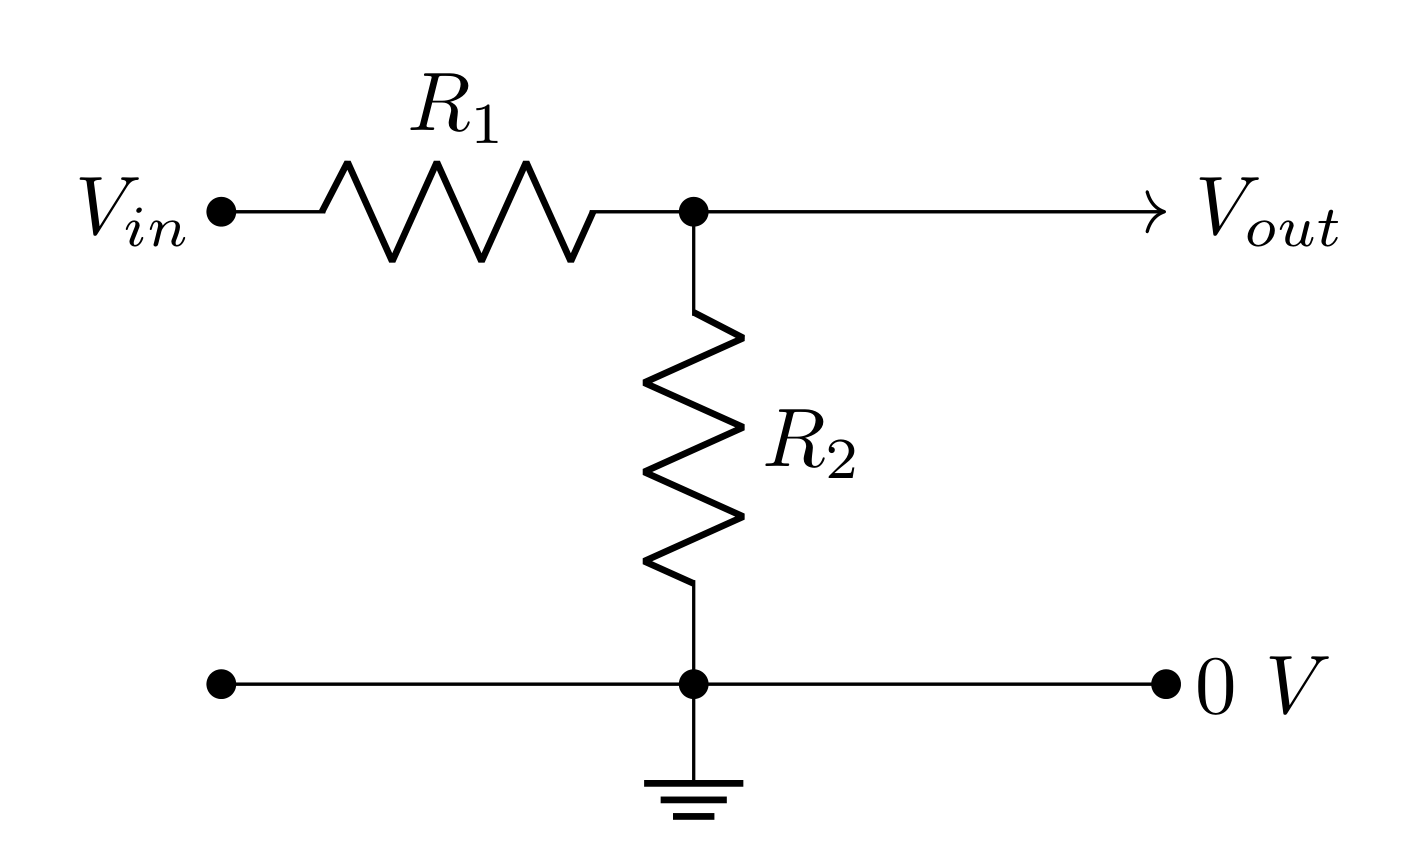
\includegraphics[width=7cm]{lab3fig/r-divider.png} }\label{r-divider}}%
%     \subfloat[\centering Low-pass filter]{{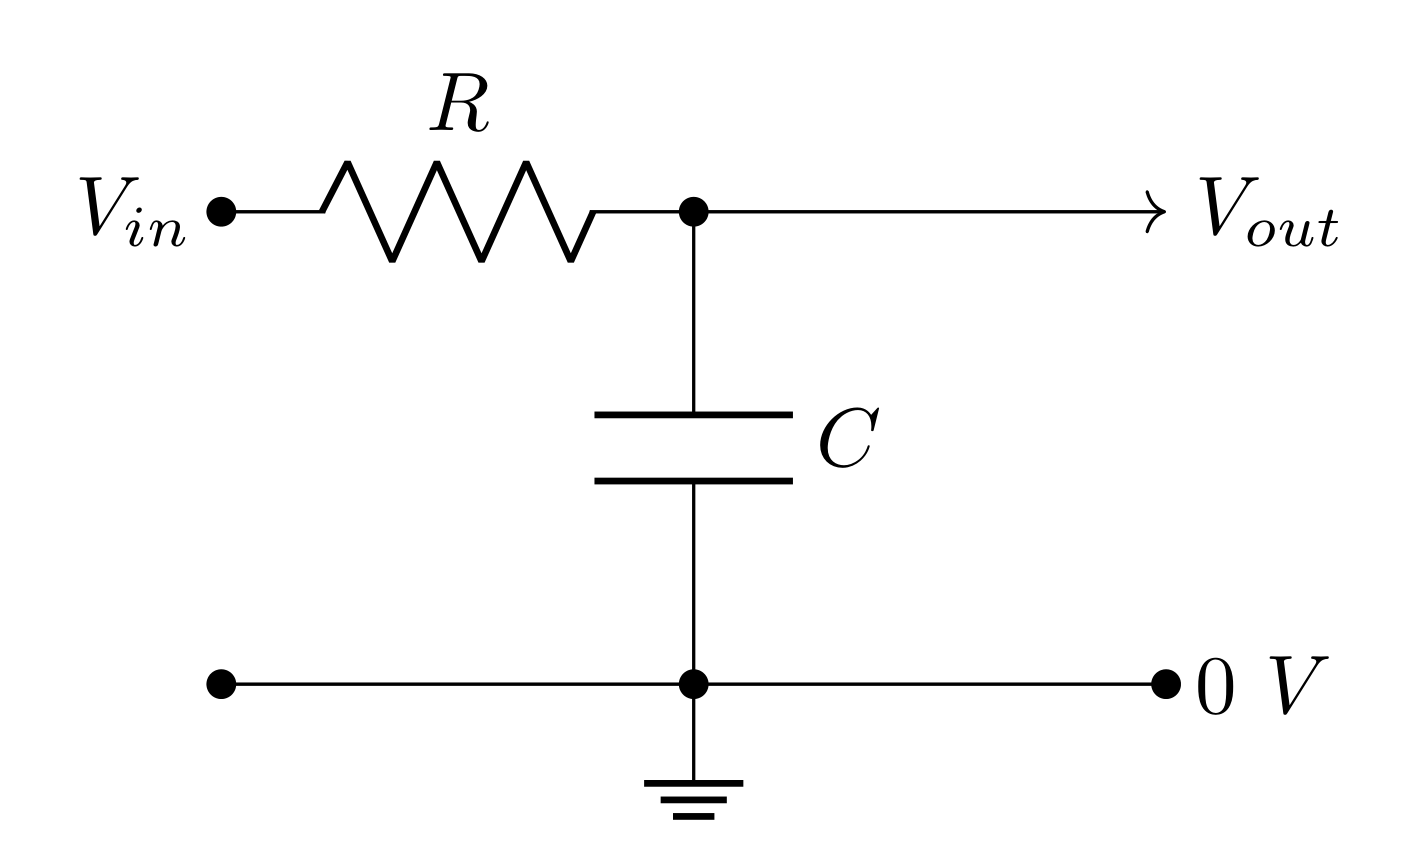
\includegraphics[width=7cm]{lab3fig/low-pass-2.png} } \label{low-pass-2}}\\%
%     \subfloat[\centering High-pass filter]{{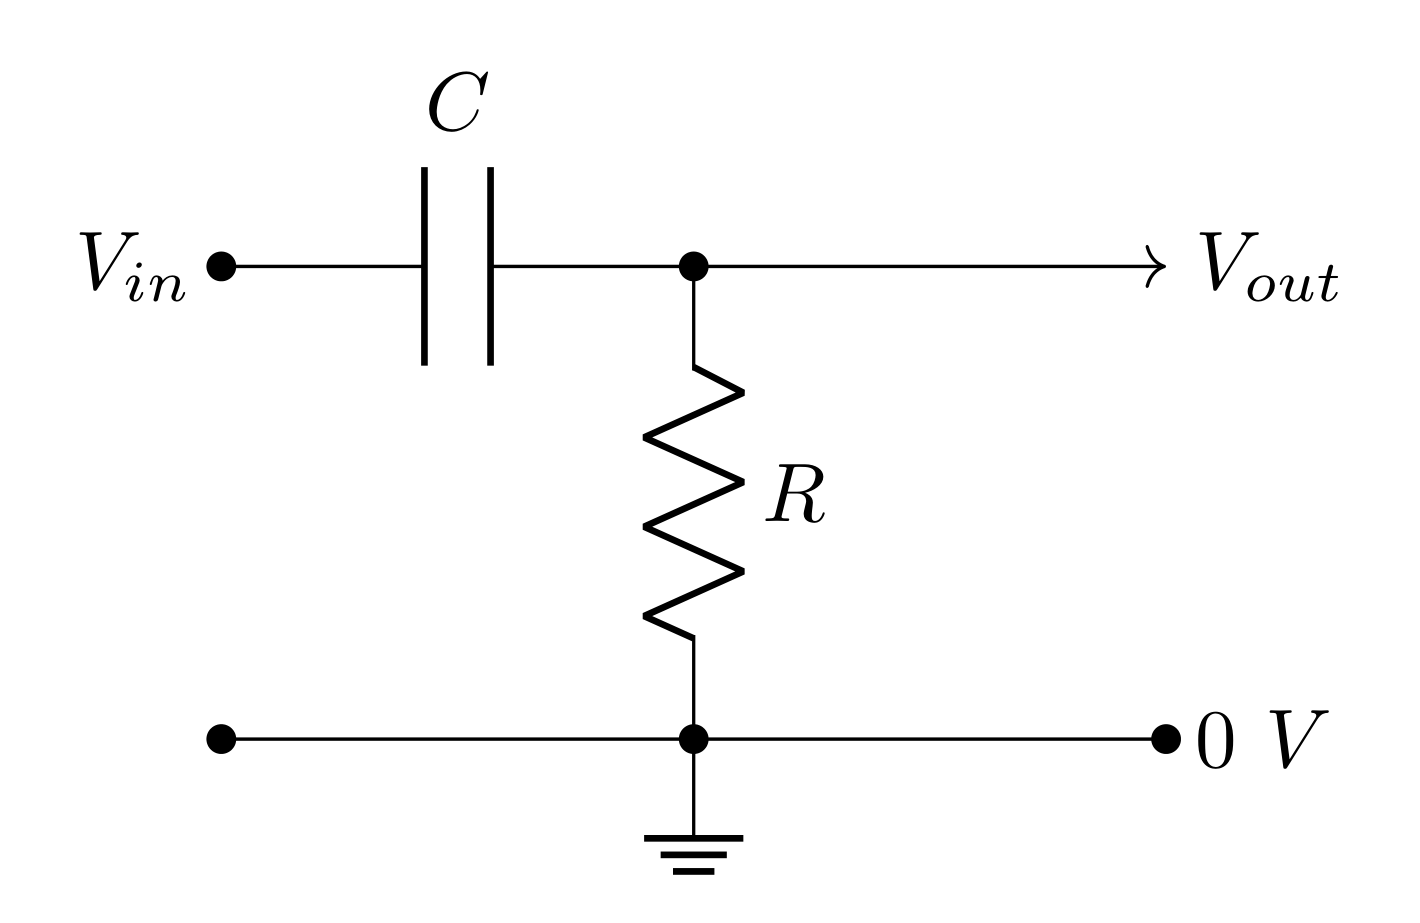
\includegraphics[width=7cm]{lab3fig/high-pass-2.png} }\label{high-pass-2}}%
%     \subfloat[\centering Band-pass filter]{{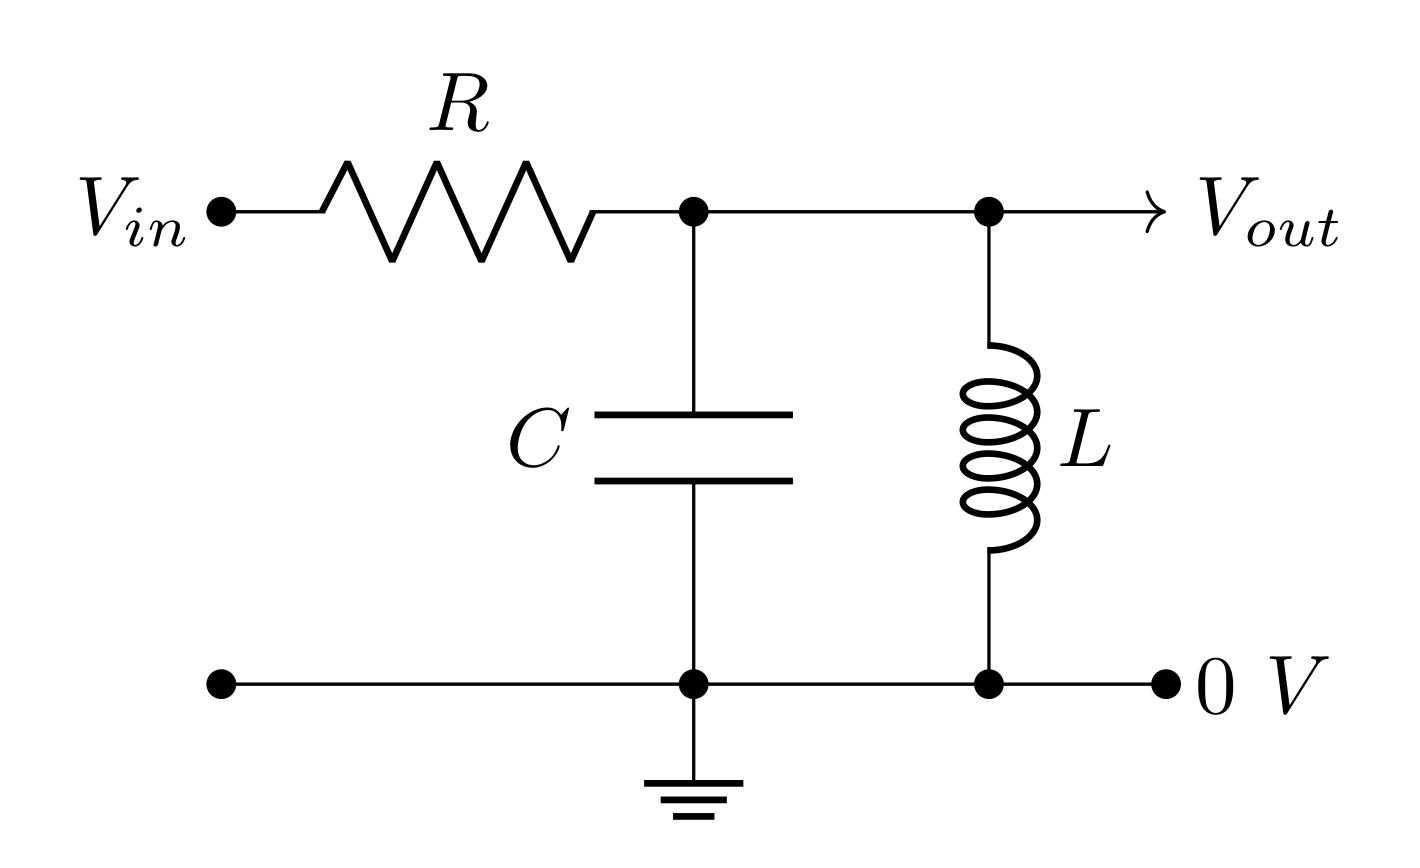
\includegraphics[width=7cm]{lab3fig/band-pass-2.png} }\label{band-pass-2}}%
%     \medskip
%     \caption{Filters}%
%     \label{dividers}%
% \end{figure}



\begin{figure}[ht]
\centering
\begin{subfigure}[t]{0.3\textwidth}
\centering
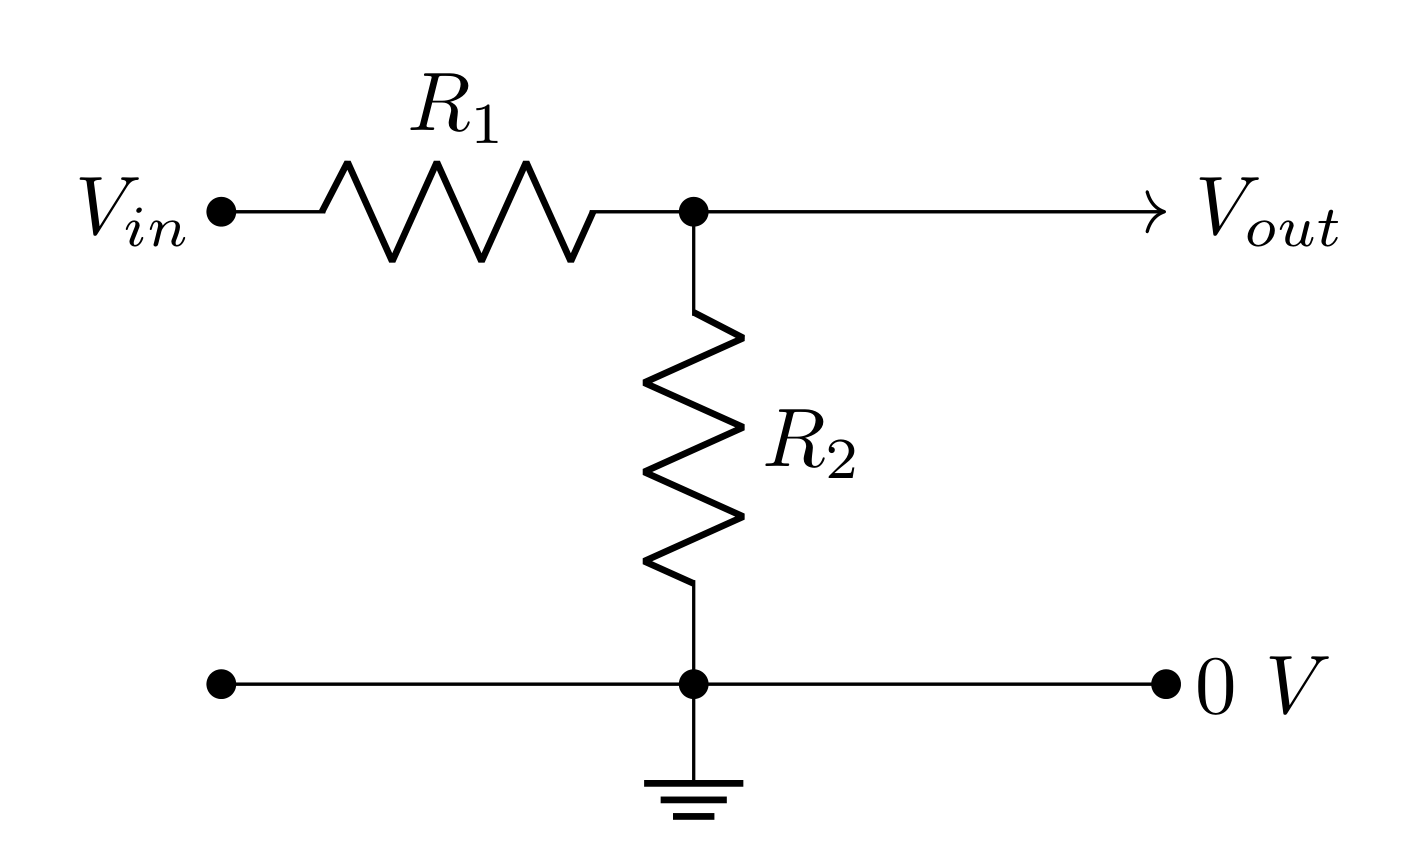
\includegraphics[width=\textwidth]{lab3fig/r-divider.png}

 \caption{resistive divider}
 \label{r-divider}
 \end{subfigure}
 \hspace{1.1cm}%
 \begin{subfigure}[t]{0.3\textwidth}
\centering
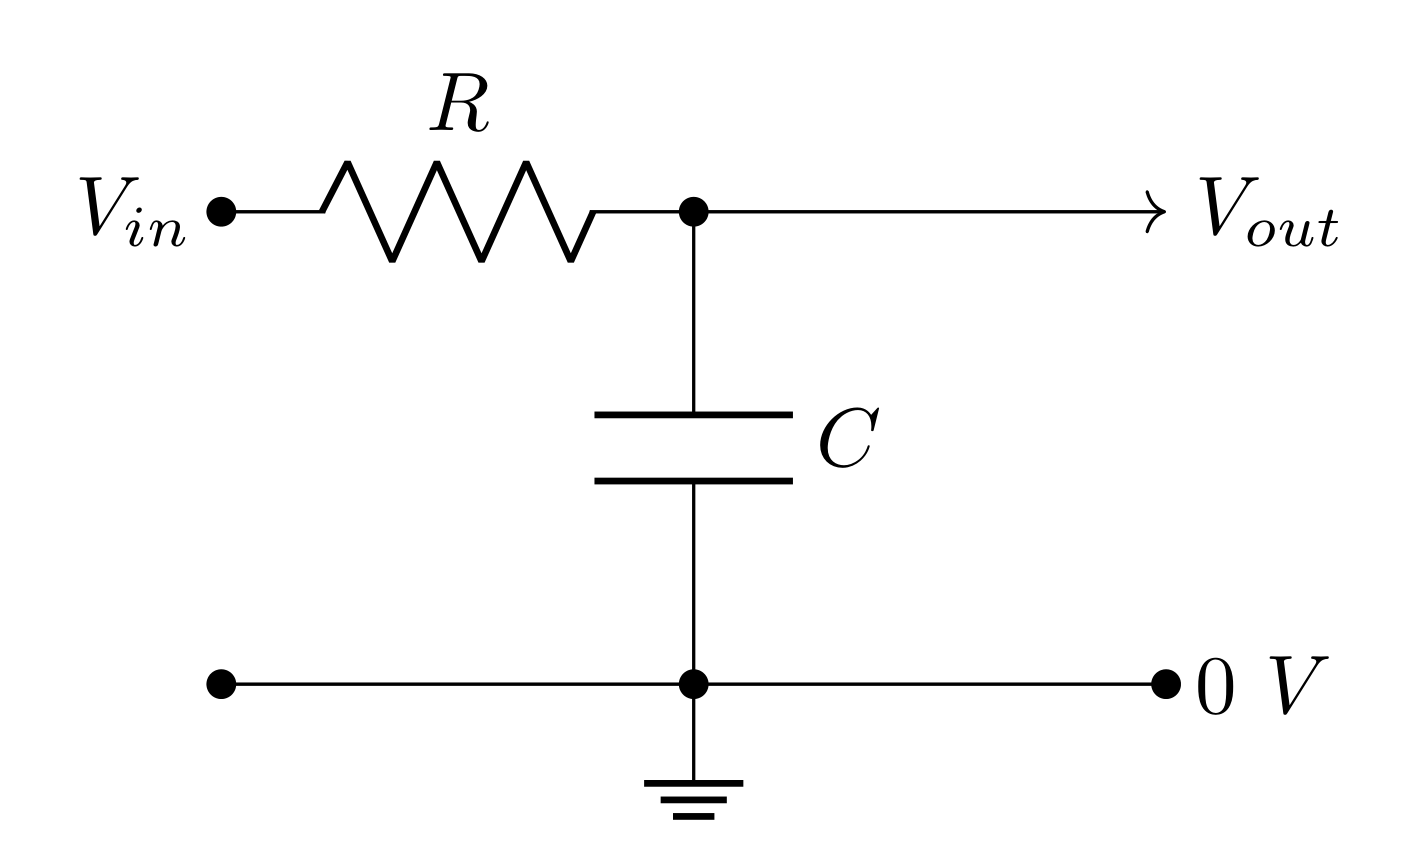
\includegraphics[width=\textwidth]{lab3fig/low-pass-2.png}

 \caption{low-pass filter}
 \label{low-pass-2}
 \end{subfigure}\\
 %\hspace{1.1cm}%
 \medskip
 \begin{subfigure}[t]{0.3\textwidth}
 \centering
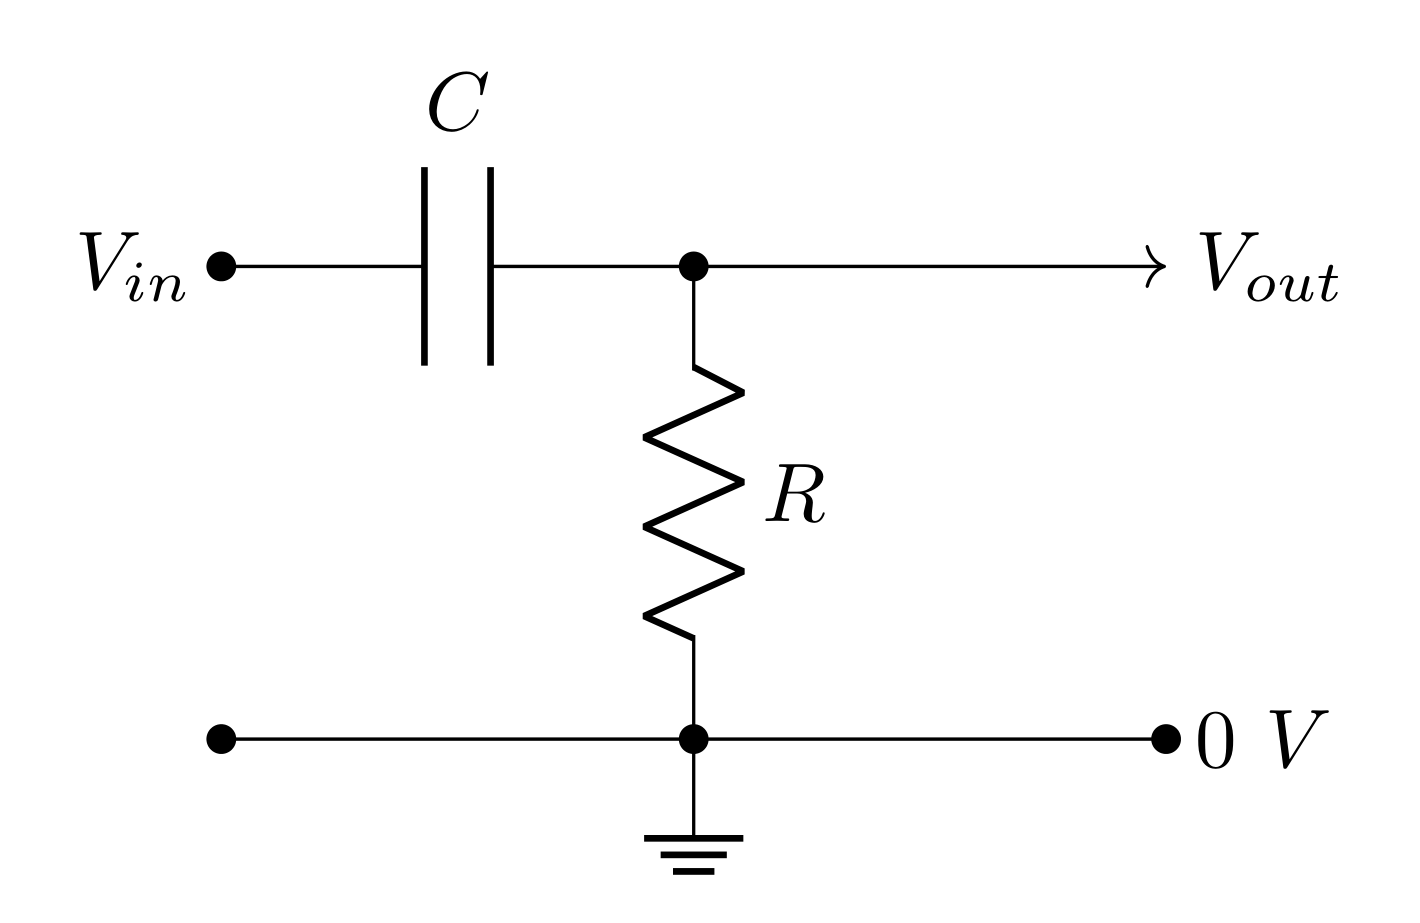
\includegraphics[width=\textwidth]{lab3fig/high-pass-2.png}

 \caption{high-pass filter}
 \label{high-pass-2}
 \end{subfigure}
\hspace{1.1cm}%
 \begin{subfigure}[t]{0.3\textwidth}
\centering
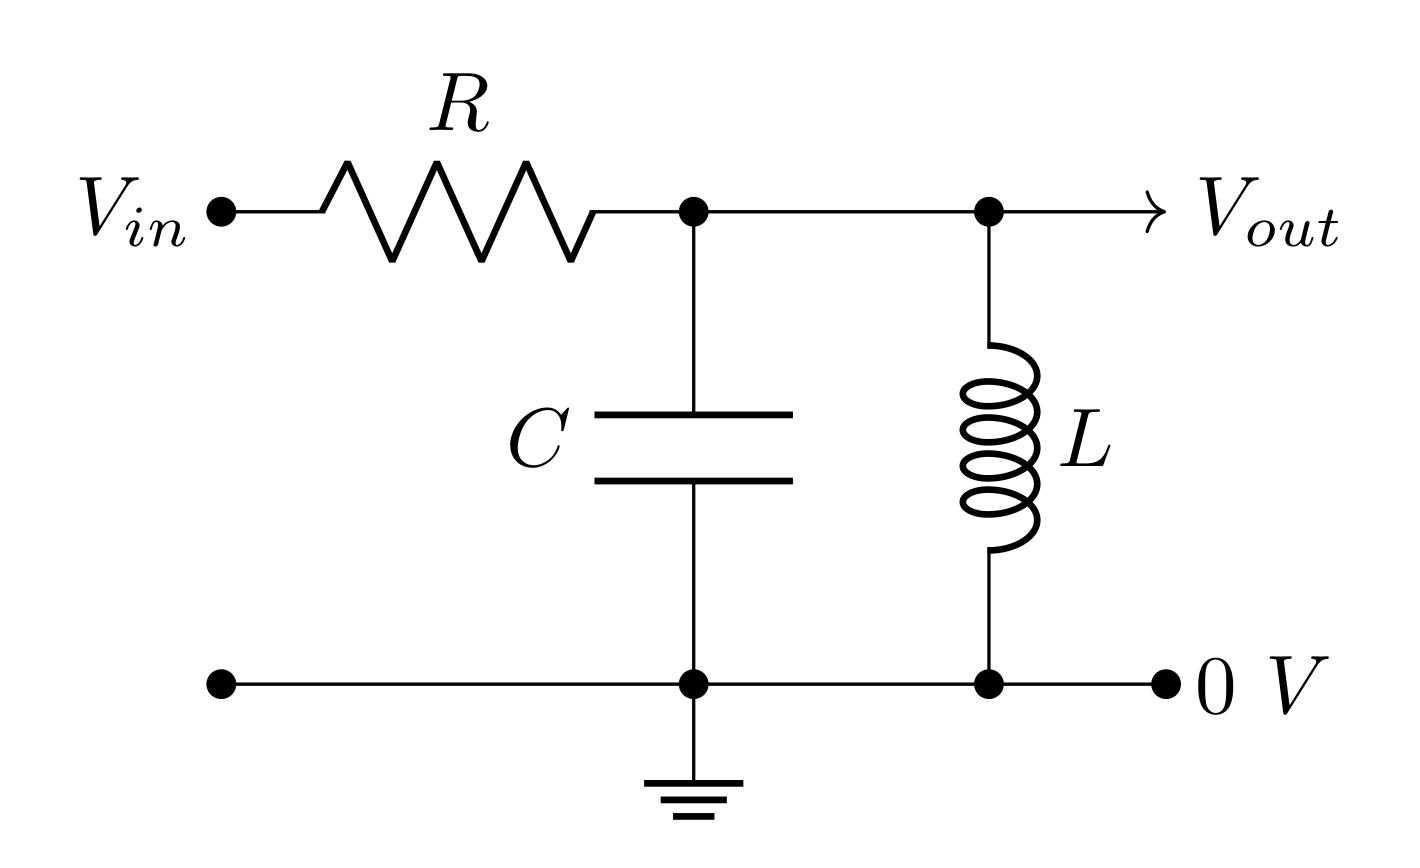
\includegraphics[width=\textwidth]{lab3fig/band-pass-2.png}

 \caption{band-pass filter}
 \label{band-pass-2}
 \end{subfigure}
  \medskip
 \caption{General Voltage Dividers}
 \label{dividers}
 \end{figure}

% \begin{figure}[ht]
% \centering
% \begin{subfigure}[t]{0.3\textwidth}
% \centering
% \begin{circuitikz}[american voltages]
%     \draw (0,0) node[anchor = east]{$V_{in}$} to [R=$R$, l=$R_1$, *-*] ++(2,0) node{}
%         [->] (2,0) to ++(2,0) node[anchor = west]{$V_{out}$};
%     \draw (2,0) to [R=$R$, l=$R_2$, -*] (2,-2) node[ground]{};
%     \draw [short,*-] (0,-2) to (2,-2)
%         to [short,-*](4,-2) node[anchor = west]{$0~V$};
% \end{circuitikz}
%  \caption{resistive divider}
%  \label{r-divider}
%  \end{subfigure}
%  \hspace{1.1cm}%
%  \begin{subfigure}[t]{0.3\textwidth}
% \centering
% \begin{circuitikz}[american voltages]
%     \draw (0,0) node[anchor = east]{$V_{in}$} to [R=$R$, l=$R$, *-*] ++(2,0) node{}
%         [->] (2,0) to ++(2,0) node[anchor = west]{$V_{out}$};
%     \draw (2,0) to [C=$C$, l=$C$, -*] (2,-2) node[ground]{};
%     \draw [short,*-] (0,-2) to (2,-2)
%         to [short,-*](4,-2) node[anchor = west]{$0~V$};
% \end{circuitikz}
%  \caption{low-pass filter}
%  \label{low-pass-2}
%  \end{subfigure}\\
%  %\hspace{1.1cm}%
%  \medskip
%  \begin{subfigure}[t]{0.3\textwidth}
%  \centering
% \begin{circuitikz}[american voltages]
%     \draw (0,0) node[anchor = east]{$V_{in}$} to [C=$C$, l=$C$, *-*] ++(2,0)
%     [->] (2,0) to ++(2,0) node[anchor = west]{$V_{out}$};
%     \draw (2,0) to [R=$R$, l=$R$, -*] (2,-2) node[ground]{};
%     \draw [short,*-] (0,-2) to (2,-2)
%         to [short,-*](4,-2) node[anchor = west]{$0~V$};
% \end{circuitikz}
%  \caption{high-pass filter}
%  \label{high-pass-2}
%  \end{subfigure}
% \hspace{1.1cm}%
%  \begin{subfigure}[t]{0.3\textwidth}
% \centering
% \begin{circuitikz}[american voltages]
%     \draw (0,0) node[anchor = east]{$V_{in}$} to [R=$R$, l=$R$, *-*] ++(2,0) node{}
%         [->] (2,0) to ++(2,0) node[anchor = west]{$V_{out}$};
%     \draw (2,0) to [C=$C$, l_=$C$, -*] (2,-2) node[ground]{};
%     \draw [short,*-] (0,-2) to (2,-2)
%         to [short,-*](4,-2) node[anchor = west]{$0~V$};
%     \draw (3.25,0) to [L=$L$, *-*] (3.25,-2);
% \end{circuitikz}
%  \caption{band-pass filter}
%  \label{band-pass-2}
%  \end{subfigure}
%   \medskip
%  \caption{General Voltage Dividers}
%  \label{dividers}
%  \end{figure}


\subsection{Building the Circuits}


\begin{enumerate}
\def\labelenumi{\arabic{enumi}.}
\item
  Gather all the components to be able to build the three filters
  circuits shown in Figure \ref{dividers}. If you cannot find components in stock with
  the specified values, take the nearest in value that you can find.

  \begin{itemize}
  \item
    Low-pass filter: $R = 10~k\Omega$, $C = 1000~pF$
  \item
    High-pass filter: $R = 10~k\Omega$, $C = 1000~pF$
  \item
    Band-pass filter: $R = 10~k\Omega$, $C = .01~\mu F$, $L = 10~mH$
  \end{itemize}
\item
  Measure all components before placing them into the circuit. Record
  the values in your lab notebook. Draw diagrams of all the circuits.
  Make sure to use the same labels on the diagrams and for the values of
  the components.
\item
  Build all three circuits on your breadboard (make sure they are all
  separate). Don't connect anything to power or ground yet. Note that
  the inductor leads are a bit thick. It is probably OK to give it a
  little force but you can also use wires with alligator clips (with
  regular wires on the other ends) to make the connections.
\end{enumerate}

\subsection{Use the Mathematica models to predict the behavior of the filters}


\begin{enumerate}
\def\labelenumi{\arabic{enumi}.}
\item
  Calculate the expected values of the cut-off frequencies for the high-
  and low-pass filters using the actual component values.
\item
  Calculate the expected resonant frequency \(f_0\) and quality factor
  \(Q\) for the band-pass filter using the actual component values.
\end{enumerate}

\emph{HINT: You should have already done these calculations in your lab
prep notebook. Just enter the measured values of your components.}

\subsection{Use the Mathematica models to plot the expected the behavior of the filters}


Plot your mathematical models of all three filter circuits (three
independent plots) using your actual component values. The frequency
range should cover at least \(10^{–3}  f_c\) to \(10^3 f_c\) (or
\(f_0\)) to show the full behavior.

\emph{HINT: You should have already made these plots in your lab prep
notebook. Just enter the measured values of your components.}

\begin{figure}[h]\centering
    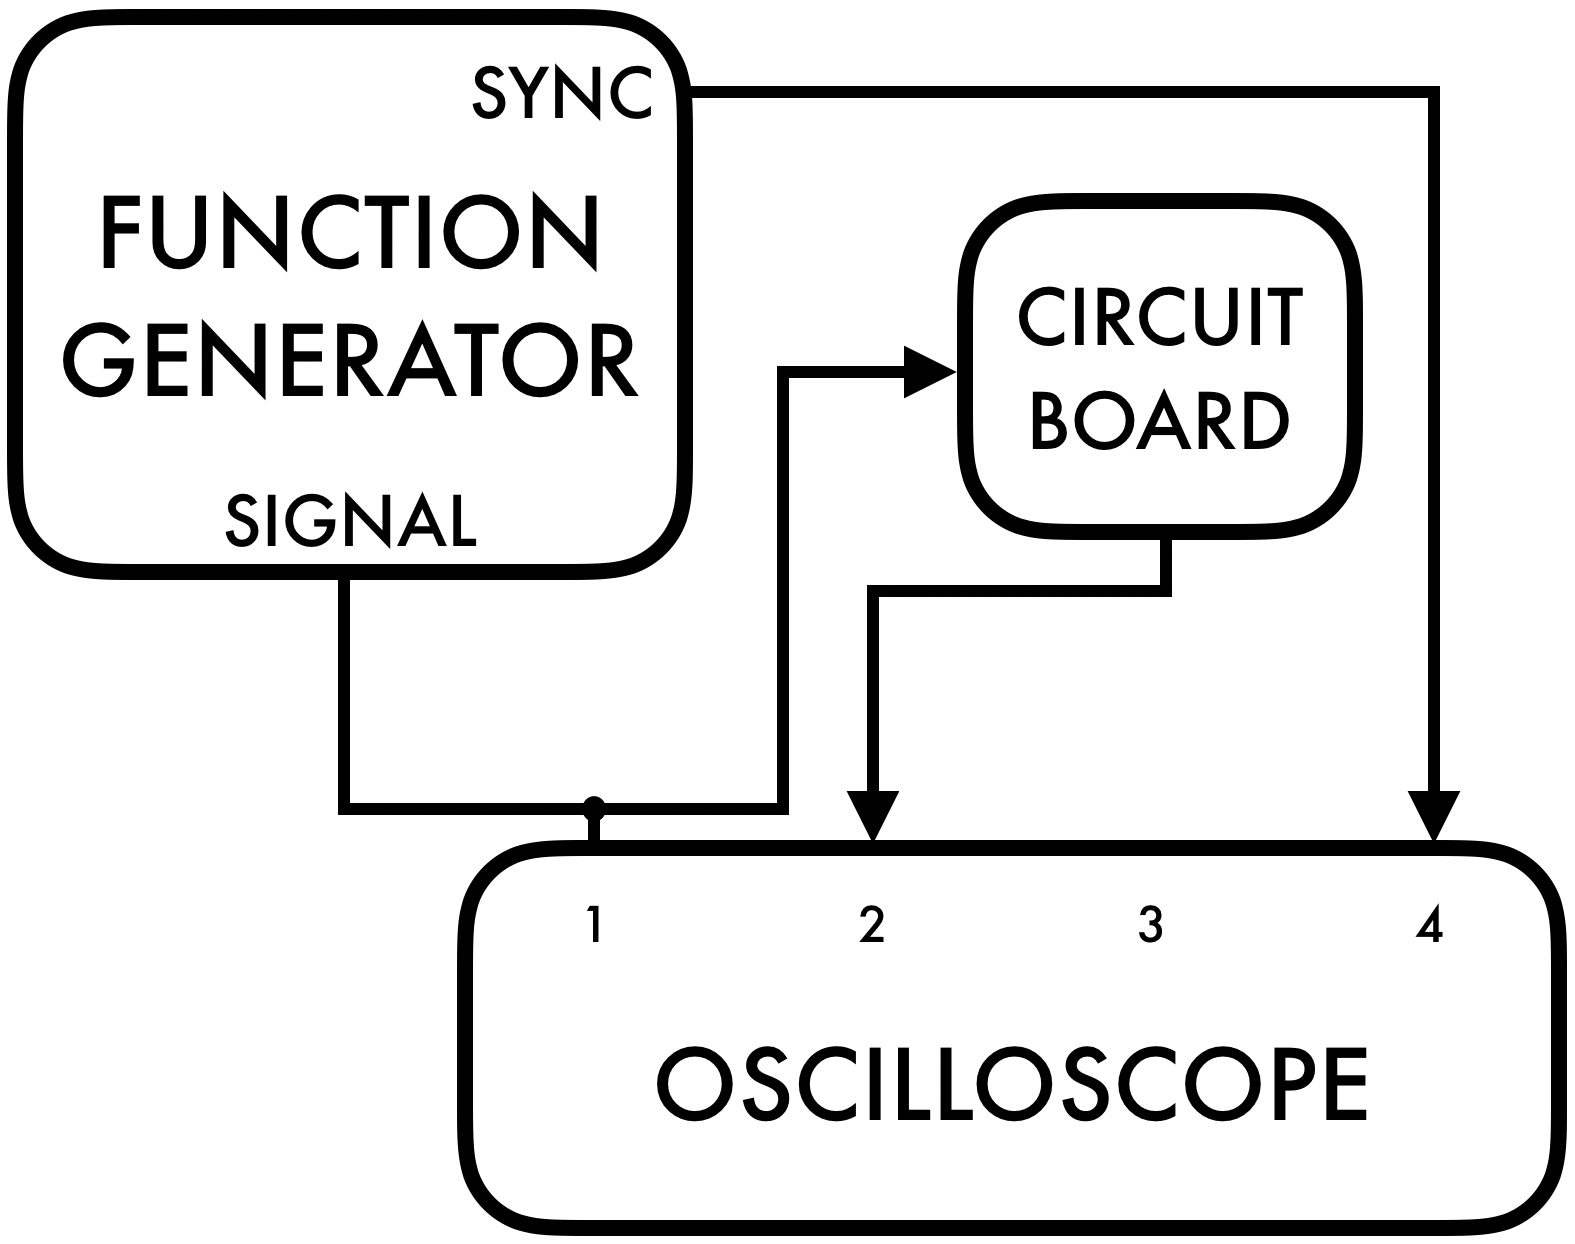
\includegraphics[width=10cm]{lab3fig/equip-setup.png}
    \caption{Test and Measurement Set-up. Channel 1 will ``pick
off'' the function generator signal on its way to the circuit board. You
can do this using a BNC ``T'' connector mounted directly on the
oscilloscope input. When you connect the oscilloscope like this, you
need to make sure the channel impedance is set to high impedance (not $50 \Omega$).}
    \label{setup}
\end{figure}


%------------------------------------------------

\section{Setting Up Test and Measurement Equipment and Testing Your Circuits}

\subsection{Prepare to test the circuits}


\begin{enumerate}
\def\labelenumi{\arabic{enumi}.}
\item
  Connect the circuit board to the function generator and the
  oscilloscope as shown in Figure \ref{setup}. It is always helpful to display both
  the input voltage as well as the output voltage on the scope at the
  same time.
\item
  Test your setup by creating a 1 kHz sine wave at 1 V p-p using the
  function generator and confirm the waveform frequency and amplitude by
  measuring the signal on the scope.
\end{enumerate}


\subsection{Measure the frequency dependence of the low- and high-pass filters}


\begin{enumerate}
\def\labelenumi{\arabic{enumi}.}
\item
  Connect the signal from the function generator to the input of the
  low-pass filter. Measure the transfer function (\(|V_{out}/V_{in}|\))
  over a large range in frequency (100 Hz to 1 MHz) in at least one step
  per decade, with several extra steps within the decade around your
  expected cutoff frequency. Record your measurements in your lab
  notebook. Determine and record the cut-off frequency for the low-pass
  filter. Compare your measured half power point
  (\(|V_{out}/V_{in}|=0.707\)) with the cut-off frequency computed from
  the actual component values used. Include your comparison in your lab
  notebook. Then do the same for the high-pass filter.
\item
  Test the predicted frequency response by plotting your data points
  directly on your two Bode plots. Does the model agree with your data?
  Explicitly record what criteria you used to determine whether or not
  the model and measurements agree.
\end{enumerate}

\subsection{Measure the frequency dependence of the band-pass filter}


\begin{enumerate}
\def\labelenumi{\arabic{enumi}.}
\item
  When the input frequency is at the resonance value $f_0$, $V_{out}$ will be a
  maximum and the phase shift between the input and output waveforms
  will be zero. This gives you two ways to find the resonant frequency.
  Find the resonant frequency $f_0$ both ways. That is, adjust the
  frequency so that (1) \(|V_{out}/V_{in}|\) is a maximum, and (2) there
  is zero phase difference between \(V_{out}\) and \(V_{in}\). Record
  both measurements of \(f_0\). Which method is more precise? Explain
  why you think so. \emph{Hint: try to estimate the uncertainty in both
  cases.}
\item
  The LCR meter measured the inductance of your inductor at a particular
  frequency. Your inductor's inductance changes slightly at different
  frequencies. Use your measurement of \(f_0\) to get a more accurate
  measure of \(L\) on resonance by doing the following. Compare the
  measured \(f_0\) with the expected value \(1/(2\sqrt{LC})\). Refine
  the model of the inductor by calculating a corrected value of \(L\)
  from the measured values of \(f_0\) and \(C\), and use this refined
  value below. Compare this value to the value you measured using the
  LCR meter in the lab.
\item
  Determine the quality factor \(Q\) by measuring the frequencies at the
  two half-power points \(f_+\) and \(f_–\). Record your measurements.
  Recall that \(Q=f_0/\Delta f\) where \(\Delta f=f_+-f_-\). \emph{Hint:
  The half-power points are where \(V_{out}=V_{out}(max)/\sqrt 2\), not
  \(V_{in}/\sqrt 2\).}
\item
  Compare the measured value of \(Q\) with your predicted value. Do they
  agree?
\item
  It is common in all electrical circuits to find \(Q\) values that are
  somewhat lower than values you predict. This is due to additional
  losses in the circuit. In this case the losses are primarily in the
  inductor. Measure the inductor's ``equivalent series resistance''
  (ESR) using a DMM. You can refine your model by including this
  resistance in your circuit. Draw a schematic that includes this
  resistor. What is the predicted \(Q\) when you include this resistance
  in your model? \emph{See Appendix A. Does this result in
  better agreement with your measured \(Q\)?}
\item
  Measure the gain (\(|V_{out}/V_{in}|\)) as function of frequency. Use
  your model prediction to decide what values of frequency to take data.
  Plot your measurements on the same graph as your model. Does your data
  match your model prediction? Note, your transfer function did not
  include the refined value of \(Q\).
\end{enumerate}

%------------------------------------------------

\section{Summary and Conclusions}

Write a two-paragraph summary in your lab notebook of what you learned
and any important takeaways.

%------------------------------------------------

\section*{Appendix A: Refined LCR Band-Pass Filter Model}

\addcontentsline{toc}{section}{Appendix A: Refined LCR Band-Pass Filter Model} % Adds this section to the table of contents


Inductors often have considerable resistance as they are just wires
wrapped around a ferrite core. One can include this resistance as a
resistor in series with the inductor. The refined model of the Q of this
system is

\[Q_{refined} = \frac{\frac{R}{R_{L}}}{R\sqrt{\frac{C}{L}} + \frac{1}{R_{L}}\sqrt{\frac{L}{C}}}\]

where \(R_L\) is the equivalent series resistance of the inductor. This
is non-trivial to derive.
%------------------------------------------------


\end{document}